\documentclass[tikz, border=5mm]{article}
\usepackage{pgfplots}
\usepackage{amsmath}

\begin{document}

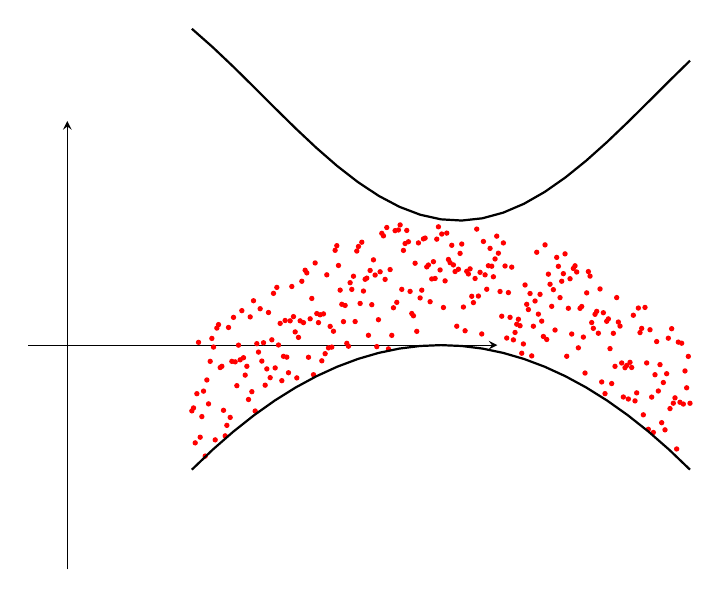
\begin{tikzpicture}[
    declare function={a(\x)=-(0.5*\x-1.5)^2+1;},
    declare function={b(\x)=-(0.5*\x-1.5)^2;},
    declare function={f1(\x)=2+cos(\x*57.3)*1;}
]
\begin{axis}[
    domain=1:5,
    xmin=0,
    ymin=-1.5,
    xmax=3.14,
    ymax=1.5,
    axis lines=middle,
    axis equal image,
    xtick=\empty, 
    ytick=\empty,
    enlargelimits=true,
    clip mode=individual, 
    clip=false,
    xlabel=\empty,%{\Large{$\widehat{Y}$}}, xlabel style={at=(xticklabel cs:1.05), anchor=north west},
    ylabel=\empty,%{\Large{$e$}}, ylabel style={at=(yticklabel cs:1), anchor=south east},
]
\addplot [red, only marks, mark=*, samples=300, mark size=0.75]
    {0.5*(a(x)+b(x)) + 0.5*rand*(a(x)-b(x))};
\addplot [thick] {f1(x)};
\addplot [thick] {b(x)};
\end{axis}
\end{tikzpicture}

\end{document}